\documentclass[12pt]{article}

\usepackage[utf8]{inputenc}
\usepackage[T1]{fontenc}
\usepackage[spanish]{babel}
\usepackage{cmbright}
\usepackage{lmodern}
\usepackage{geometry}
\usepackage{pgfplots}
\usepackage{tikz}
\usetikzlibrary{positioning,calc,math,arrows.meta,decorations.markings,intersections}
\usepackage{hyperref}
\usepackage[bf,sf,pagestyles]{titlesec}
\usepackage{titling}
\usepackage[runin]{abstract}
\usepackage[font={footnotesize, sf}, labelfont=bf]{caption} 
\usepackage{siunitx}
\usepackage{graphicx}
\usepackage{booktabs}
\usepackage{amsmath,amssymb}
\usepackage[spanish,sort]{cleveref}
\usepackage{enumitem}

\geometry{
	a4paper,
	right = 2.5cm,
	left = 2.5cm,
	bottom = 3cm,
	top = 3cm
}

\newcommand{\sfbright}{\fontfamily{cmbr}\selectfont}
\renewcommand{\familydefault}{\rmdefault}
\renewcommand{\sfdefault}{cmbr}
\renewcommand{\arraystretch}{1.4}

\hypersetup{
	colorlinks,
	linkcolor = {red!50!blue},
	citecolor = {red!50!blue},
	linktoc = page
}

\numberwithin{table}{section}
\numberwithin{figure}{section}
\numberwithin{equation}{section}

\graphicspath{{./figs/}}

% Unitats
\sisetup{
	inter-unit-product = \ensuremath{ \, },
	allow-number-unit-breaks = true,
	math-celsius = {}^{\circ}\kern-\scriptspace C,
	detect-family = true,
	mode = text,
	list-final-separator = { y },
	list-pair-separator = { y },
	list-units = single,
	separate-uncertainty = true
}

\newcommand{\Z}{\mathbb{Z}}
\newcommand{\N}{\mathbb{N}}
\newcommand{\R}{\mathbb{R}}
\newcommand{\Ry}{\mathit{Ry}}
\newcommand{\conv}[2]{\filldraw[fill = white!50!-red, fill opacity = 0.5, draw = -red!] (#1,0) ellipse [x radius = 0.1, y radius = #2];}
\newcommand{\data}[3]{\SI{#1 \pm #2}{#3}}
\newcommand{\unc}[2]{\ensuremath{{}\pm \SI{#1}{#2}}}
\DeclareMathOperator{\gr}{gr}
\newcommand{\abs}[1]{\left\lvert #1 \right\rvert}
\newcommand{\inn}[2]{\left\langle #1 , #2 \right\rangle}
\newcommand{\parbreak}{
	\begin{center}
		--- $\ast$ ---
	\end{center} 
}
\makeatletter
\newcommand*{\defeq}{\mathrel{\rlap{%
			\raisebox{0.3ex}{$\m@th\cdot$}}%
		\raisebox{-0.3ex}{$\m@th\cdot$}}%
	=
}
\makeatother

\newpagestyle{pagina}{
	\headrule
	\sethead*{\sffamily \bfseries Práctica 5}{}{\theauthor}
	\footrule
	\setfoot*{}{}{\sffamily \thepage}
}
\renewpagestyle{plain}{
	\footrule
	\setfoot*{}{}{\sffamily \thepage}
}
\pagestyle{pagina}

\title{\sffamily {\bfseries Práctica 5:} Polarización de la luz}
\author{\sffamily B2 2: Arnau Mas, Alejandro Plaza}
\date{\sffamily 28 de marzo de 2019}

\begin{document}
\maketitle
\renewcommand{\abstractname}{\sffamily \bfseries Resumen:}
\begin{abstract}
Abstract aquí
\end{abstract}
\hrule

\section{Objetivos}
En esta práctica se pretende estudiar el fenómeno de la polarización de la luz, ---que muestra que la luz es una onda transversal---, y diversos modos de causarlo.

Se estudiará la polarización por absorción selectiva de diversos materiales, por reflexión, por dispersión Rayleigh en la luz proveniente del cielo y por birrefringencia en láminas retardadoras.

Por último se comprobará la ley de Malus para la intensidad de luz que atraviesa dos polaroides.

\section{Polarización por dicroísmo}
La polarización por dicroísmo tiene lugar cuando la luz atraviesa una lámina de un material que absorbe una componente y transmite la perpendicular. Normalmente estas láminas consisten en cadenas rectilíneas de moléculas que permiten a los electrones moverse en una sola dirección. Si esta dirección es la vertical, los electrones interactuarán con la componente de la onda cuyo campo eléctrico oscile en el eje vertical, pues el que oscila en el eje horizontal no puede ejercer trabajo sobre los electrones, ya que estos no se desplazan en la dirección horizontal. Así pues los electrones de la lámina absorben la componente vertical del campo eléctrico y transmiten la componente horizontal.

Se apunta a una pantalla con una fuente de luz y se coloca un polarizador HN-22 entre ambas. El resultado es una leve disminución de la intensidad de la luz que llega a la pantalla. Al girar el polarizador no se observa ningún cambio, pues se está cambiando la dirección de polarización de la luz que llega a la pantalla pero no su intensidad.

La disminución de intensidad es un indicio de que la luz se ha polarizado, pero no es una prueba, pues podría por ejemplo absorberse una fracción de la luz igual para todas las direcciones. Para comprobar que efectivamente la luz sale polarizada se coloca entre el polaroide y la pantalla otro polaroide HN-38. al girar el segundo polaroide la intensidad va aumentando y disminuyendo. Cuando la pantalla está oscura es porque los ejes de transmisión de ambos polaroides son perpendiculares. El primer polaroide deja pasar luz únicamente en una dirección, que es justo la dirección que absorbe el segundo. Por lo tanto no llega luz a la pantalla y se ve oscura. Sin embargo, la oscuridad no es total, ya que los polarizadores no son ideales: tansmiten un poco de luz en la dirección de absorción y viceversa. Este fenómeno pone en evidencia que la luz que sale de los polaroides está efectivamente polarizada.

Ahora se cambia el polaroide HN-38 por uno HN-22, de manera que los dos polariodes tienen las mismas curvas de transmitancias. Estas curvas se encuentran en la figura \ref{P5transmitancias}. En este caso cuando los ejes de transmisión son perpendiculares se ve una oscuridad más intensa porque la transmitancia del polaroide HN-22 en el eje de absorción es mucho menor que la del HN-38. La intensidad cuando los ejes son paralelos es parecida con el polaroide HN-38 y el HN-22 porque tienen transmitancias similares en el eje de transmisión.

\begin{figure}[!ht]
\begin{center}
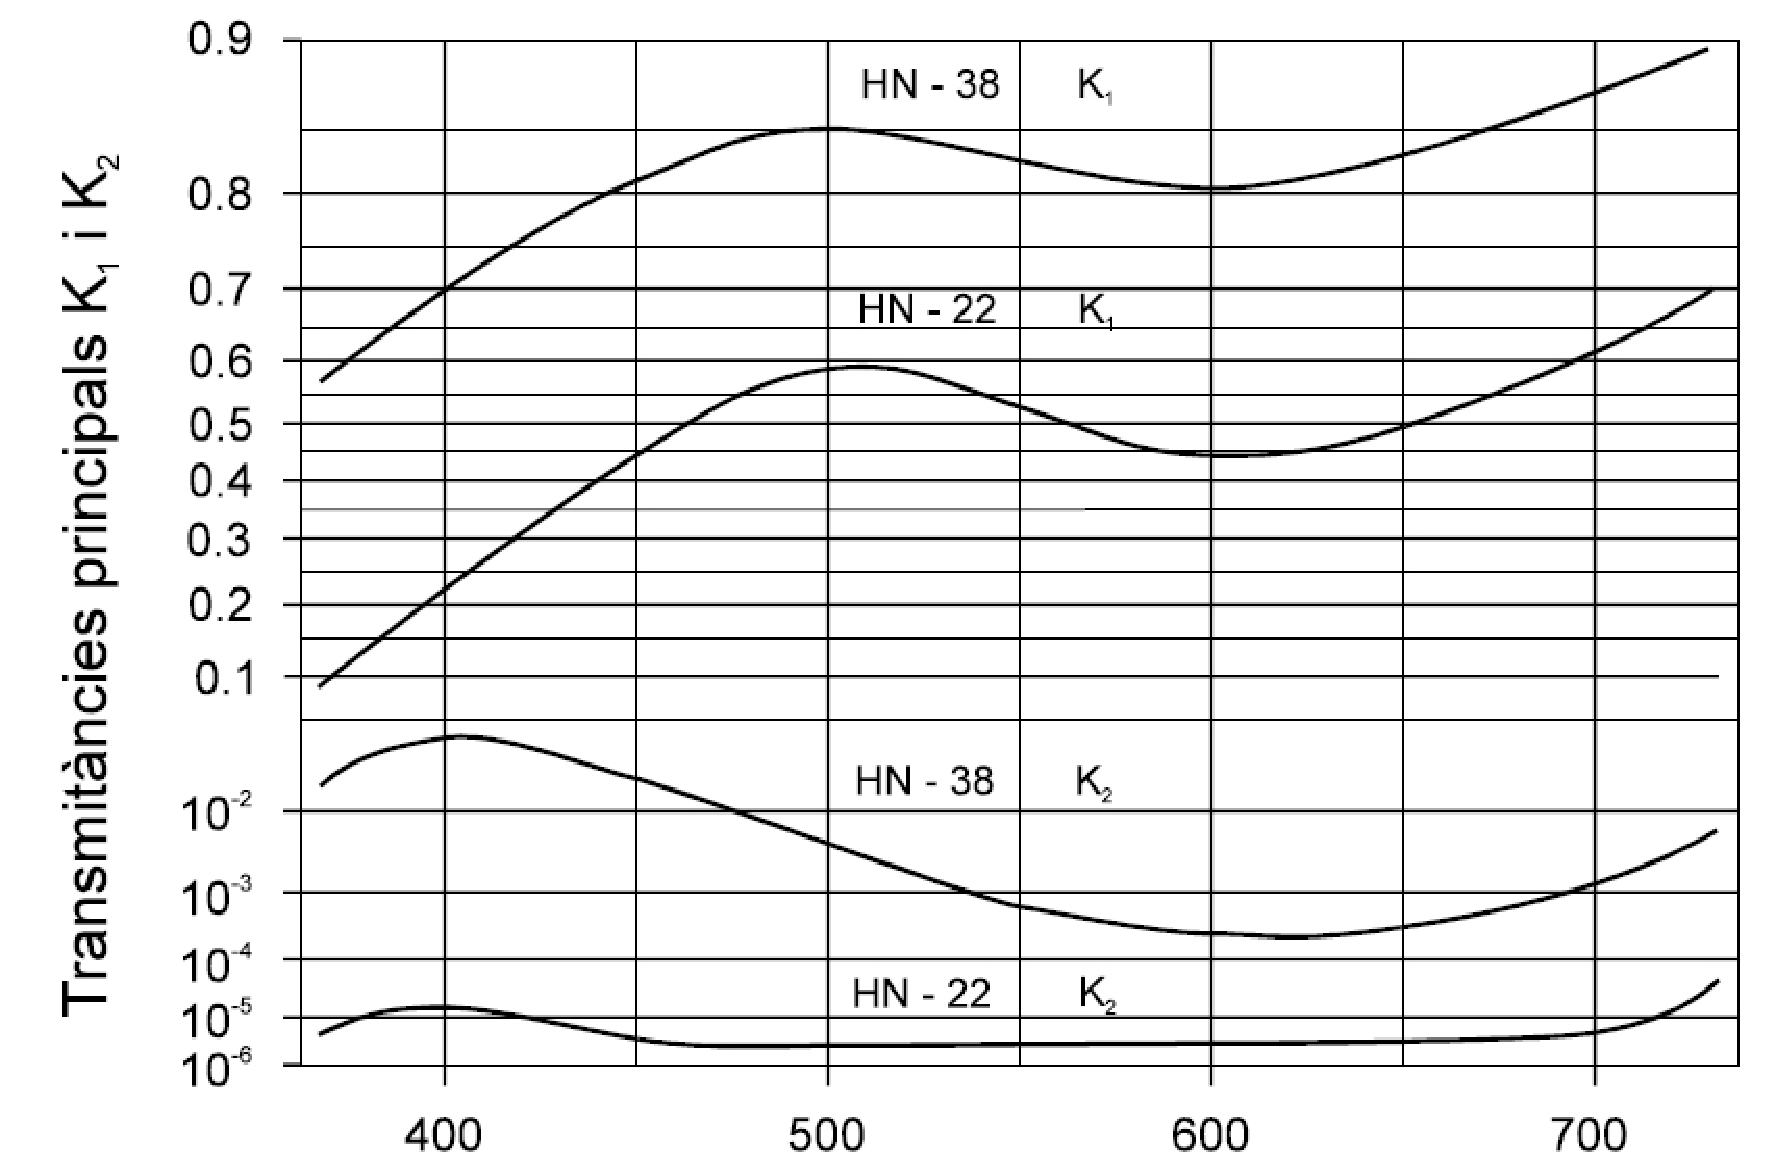
\includegraphics[width=10cm]{P5Transmitancias.pdf}
\caption{Gráficas de las transmitancias principales $K_1$ y $K_2$ en los ejes de transmisión y absorción respectivamente de los polarizadores HN-22 y HN-38 en función de la longitud de onda.}\label{P5transmitancias}
\end{center}
\end{figure}

Uno de los polarizadores tiene el eje de transmisión marcado. El eje de transmisión del otro se puede determinar girándolo hasta obtener la posición en la que la intensidad que llega a la pantalla es mínima. En este punto el eje de transmisión es el perpendicular al del otro polarizador ---cuyo eje de transmisión es conocido---. Este método es más preciso que girar el polarizador hasta obtener intensidad máxima ---siendo igual la dirección de transmisión de ambos polaroides--- porque se determina con mayor exactitud el ángulo de intensidad mínima que la máxima.

En la figura \ref{P5transmitancias} se ve que las transmitancias dependen de la longitud de onda. Para poner de manifiesto esta dependencia se colocan un filtro verde y otro rojo en la fuente de luz. Cuando los ejes son paralelos no se ve mucha diferencia, pero cuando son perpendiculares la luz que llega a la pantalla es menos intensa con el filtro verde que con el rojo. Si observamos la curva de $K_1$ del HN-22 la transmitancia es similar para longiudes de onda alrededor de los \SI{500}{nm} (verde) y de los \SI{700}{nm} (rojo). Sin embargo $K_2$ es bastante mayor para el rojo que el verde (obsérvese que del $10^{-1}$ hacia abajo la escala es logarítmica: pequeños cambios en el eje $y$ son grandes cambios de transmitancia).

Ahora se disponen los polarizadores con los ejes de transmisión cruzados y se colocan objetos entre ambos polarizadores. Se coloca asimismo una lente para proyectar los objetos sobre la pantalla. Este sistema se llama polariscopio.

Si se pone una lámina de vidrio no ocurre nada. La luz sale del vidrio tal cual ha entrado. No cambia su polarización. Por lo tanto se ve oscura la pantalla. Si se pone papel, sin embargo, sí que se ve algo de luz porque la luz polarizada que llega al papel se dispersa en él y sale despolarizada. Así la luz que llega al segundo polarizador tiene una componente no nula en el eje de transmisión. Independientemente de la orientación del papel o de los polarizadores se ve lpantalla iluminada.

Cuando se pone celofán se ilumina la pantalla según el ángulo de orientación. Cuando se gira se puede conseguir que se ilumine la pantalla. Si se orienta para ver el máximo de intensidad, para que vuelva a dejar de pasar la luz se ha de girar 90º. Esto se explica porque el celofán cambia la orientación de la polarización de la luz, de modo que si antes llegaba la luz oscilando perpendicular al eje de transmisión del segundo polarizador, con el celofán se puede cambiar la orientación de la polarización para que la luz llegue al segundo polarizador con el campo eléctrico oscilando en la dirección de transmisión.

También se puso una pequeña lámina de plástico con varios trozos de cinta adhesiva simple. Se observaron los distintos trozos de diferentes colores como muestra la figura \ref{P5colorines}. El celo modifica la orientación de la polarización de la luz, pero no afecta todas las longitudes de onda por igual: cada una gira su polarización por separado. Por eso algunas longitudes de onda llegan paralelas al eje de transmisión proyectándose sobre la pantalla y otras llegan perpendiculares siendo absorbidas. Además cada capa modifica la polarización y por lo tanto según la cantidad de capas de cinta que haya se ve de un color u otro. Al girar el plástico se ve cómo cambian los colores.

\begin{figure}[!ht]
	\centering
	\begin{minipage}{0.45\textwidth}
		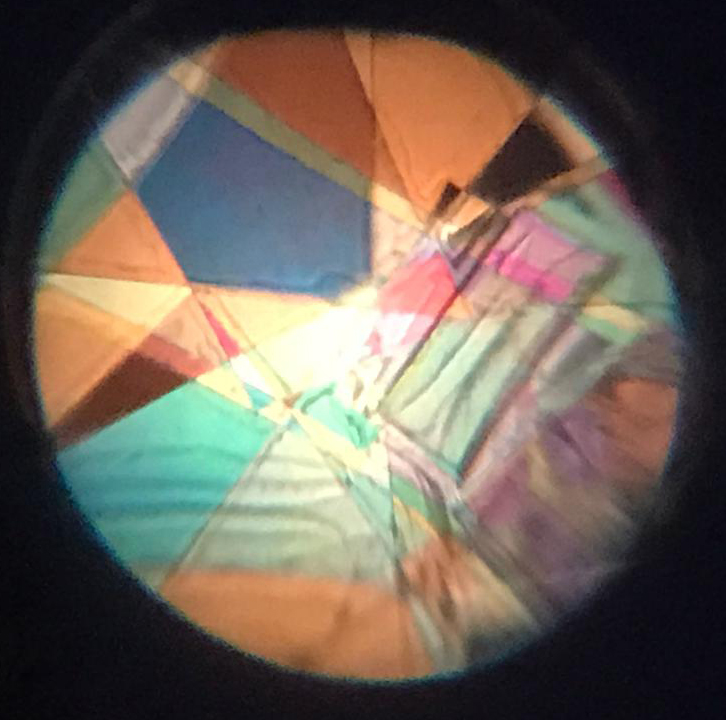
\includegraphics[scale = 0.25]{P5Celo1.jpg}
	\end{minipage}
	\begin{minipage}{0.45\textwidth}
		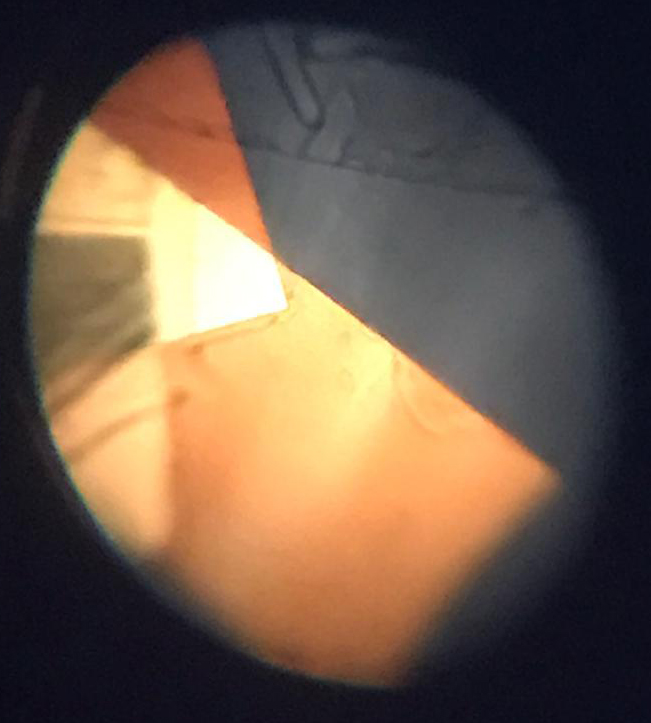
\includegraphics[scale = 0.25]{P5Celo2.jpg}
	\end{minipage}
\caption{Fotografías de la la pantalla con cinta adhesiva en el polariscopio.}\label{P5colorines}
\end{figure}

Por último se coloca una caja de un CD, que es un plástico rígido, en el polariscopio. Se observan diversos colores en la pantalla como con la cinta adhesiva. Al presionar el plástico, los colores cambian, lo cual se puede explicar porque al sufrir esfuerzos el plástico cambia la orientación de las diversas longitudes de onda de la luz polarizada.



\end{document}
